\documentclass[runningheads,a4paper]{llncs}

\usepackage{amssymb}
\setcounter{tocdepth}{3}
\usepackage{graphicx}
\usepackage{epstopdf}
\usepackage{subfig}
\usepackage{url}
\urldef{\mailsa}\path|{alfred.hofmann, ursula.barth, ingrid.haas, frank.holzwarth,|
\urldef{\mailsb}\path|anna.kramer, leonie.kunz, christine.reiss, nicole.sator,|
\urldef{\mailsc}\path|erika.siebert-cole, peter.strasser, lncs}@springer.com|
\newcommand{\keywords}[1]{\par\addvspace\baselineskip
\noindent\keywordname\enspace\ignorespaces#1}

\usepackage{todonotes}
\newcommand{\yongli}{\todo[author=YL,color=green,inline]}
%\newcommand{\naoki}{\todo[author=NK,color=yellow,inline]}

\newcommand{\eat}[1]{}
\begin{document}

\mainmatter  % start of an individual contribution

% first the title is needed
\title{Change Detection From Media Sharing Community }

% the name(s) of the author(s) follow(s) next
%
% NB: Chinese authors should write their first names(s) in front of
% their surnames. This ensures that the names appear correctly in
% the running heads and the author index.
%
\maketitle
\setcounter{section}{4}
\section{Change Detection Over Large Data Sets}\label{sec-algorithm}
In this section, we present the change detection algorithm from the large-scale social images, 
including how to identify the image pairs from the same source and how to detect the changes in images.
\subsection{Image Copy Detection}
This section presents how to effectively and efficiently identify the image pairs of the same source (same building or infrastructures etc). 
Many image copy detection approaches have been proposed and applied for various applications. 
However,  since each image may contain up to thousands of 36-dimensional local descriptors, 
directly deploying existing technique is obviously not suitable for large image databases due to the high time cost. 
To improve the efficiency of image copy identification, 
we propose a process of $SIS$-based clustering,
then deploy a PCA-SIFT-based matching over images in the same or neighboring clusters.

\subsubsection{SIS-based clustering}

Intuitively, images from the same source usually have similarity over the concept level. 
Thus it is reasonable to cluster social images based on their tag and location information, 
such that those in a single cluster or neighboring clusters will have high possibility of being from the same source. 
In this way, the identification of image copy pairs can be simplified as the comparison between images from same or neighboring clusters, 
which avoids the costly pair-wise image matching over the whole data collection. 
To do this, we need to find an efficient clustering technique that can be extended to our $SIS$ social image similarity as well. 
%Conventional clustering techniques include partitioning clustering, hierarchical clustering, overlapping clustering and subspace clustering. 
As we operate on large scale image database, the efficiency of clustering process is extremely important. 
Moreover, we only care about the similarity between images in each cluster, thus permit the overlaps between multiple ones. Thus, we extend the 2-means clustering algorithm that was initially proposed for $L_p$ distance for our $SIS$ similarity considering its low time cost as stated in \cite{DBLP:conf/sigmod/ShenZH05,DBLP:journals/tkde/ZhouZCSBT10}. 

Given an image collection, we conduct the clustering by three steps: 
1) for each image, we model its metadata as tag set and its location as a pair of latitude and longitude values;
2) we select two images with the lowest similarity as the cluster centres of two initial cluster from the current data collection. Each of the remaining images are assigned to the cluster that has the higher similarity with it. The centre points are recursively recalculated based on Equations \ref{equ:Centroid} and \ref{equ:meanLocation}, together with the images allocation to clusters based on their similarity, until the new generated centre points are stable;
3) finally, we recursively select a bigger cluster on which the second step is conducted, until the number of clusters reaches to a threshold $\kappa$.

In the social media images often there are more than 10 tags on each image and comparing these tags between the images one by one is time-consuming. 
String hashing has been applied in many applications for improving the system efficiency \cite{DBLP:conf/sigmod/ZhouCZCHW15}. 
Thus we improve our change detection efficiency by selecting a ``good'' hashing function class. 
To reduce the time expenses on tags comparison, we use the \textit{djb2} hash function techniques \cite{MartínezFE14},
which one of the best hash function techniques for the string data. 
In \textit{djb2} the hash values are populated by \textit{hash*33 + c}, 
where the hash is the long data and $c$ is the string character. 
Daniel J. Bernstein uses the magic number 33 to times the hash data, however, he did not explain why it works better than any other constants.
In our system, the \textit{djb2} is applied to all the images tags and the hash value is created for each tag. These hash values are used when the $J_t$ similarity is calculated. The first step is making the tags on the image $A$ and the image $B$ to the hash values, and then it compares the hash values of $A$ with those of $B$. Secondly, if the hash value of $A$ does not exist in that of $B$, it is considered as unmatched. As such the system does not need to compare all the string tags. This hashing reduces the total number of string comparison in the $J_t$ similarity.

\eat{
Para 1: how to choose cluster algorithm, and extend it to SIS similarity

Para 2: how to index social images for quick clustering
}

\subsubsection{PCA-SIFT-based matching} 

PCA-SIFT-based matching will be used for deciding if two image candidates are referring to the same objects. 
It will find the similarity between the objects. The main objects are the buildings, statues and other objects which are not moving. Also, the unrelated images selected by the PCA-SIFT algorithm will be removed. 
The removing occur when the images have the high $SIS$ similarity, but the images are not what the user want. The kept image pairs are passed to change detection stage for assessing if any damages had happened in a natural disaster.

We apply the OOS to the similarity calculation between the local descriptor sets of two images \cite{DBLP:journals/tmm/ZhaoNTW07}. 
Given two local interest descriptors, the similarity between them is measured by the $Cosine$ similarity between these two vectors. For two local interest points from two images, they are match pair candidate if the similarity between them is bigger than a threshold value. OOS further check if any one of these two points is the nearest neighbor of the other among all the descriptors of its image. If they are nearest neighbors of each other, they are a real matched pair. The final similarity between two images is calculated by the average similarity of all their matched pairs. To improve the local interest points matching, we use the LIP-IS index proposed in \cite{DBLP:journals/tmm/ZhaoNTW07} as well. All these ensure that effective and efficient PCA-SIFT-based matching is performed.

\subsection{Change Detection}
Change detection assesses the damages caused during disasters. Intuitively, two pictures to the same location point contains same buildings or other objects, each is described as a boundary. 
If there is no damage happened at this place, the object boundaries in two images match. 
Otherwise, if there exists boundary missing or unmatched from the before image to the after one, the damages could have be caused in the disaster. Therefore, in this section, we propose a new image object boundary modelling together with a novel boundary matching method, which are robust to different image transformations, rotations or editing, for effective change detection.

\subsubsection{Model image boundary}

Existing works model building shadow area boundaries \cite{turker2008building}, boundary shapes \cite{rs2051217} using the coordinates of each pixel falling on the boundary of objects in an image. 
However, these boundary modelling incurs low effectiveness of detection for social images because of the possible object changes with respect to the viewpoints, rotations, space shift etc. 
To address this issue, we propose a robust boundary representation, called \emph{relative position annulus} (RPA), 
which describe each boundary as an annulus of the difference of neighboring edge lengths. 
Specifically, we exploit sober edge detector to detect a number of boundaries in an image, 
since it can detect the emphasising edges while reduce the effect of noise edges. Given a boundary consisting of $m$ vertexes $\{v_1,...,v_m\}$, we represent the boundary as $\{d(v_1,v_2)-d(v_2,v_3),...,d(v_{m-2},v_{m-1})-d(v_{m-1}-v_m), d(v_{m-1},v_m)-d(v_m,v_1)\}$, where any element can be the start point while other points are ordered clockwise. As such, the RPA representation will be robust to object rotation, viewpoint change and space shift in social images.

\subsubsection{Matching boundaries}
As each image may contain multiple objects, each image is described as a set of relative position annulus of multiple boundaries. 
To assess the damages in a disaster, we need to do two steps matching: 
(1) the measure between two RPAs; 
(2) the measure between two images. 
To further reduce the influence of small noise objects, we only use the top $\kappa$ biggest boundaries for boundary comparison between two images.

Given two RPAs, $\mathcal{Q}: <q_1, q_2,...,q_m>$ and $\mathcal{D}: <v_1,v_2,...,v_{n}>$ , we measure the similarity between them by extending the DTW \cite{Berndt:1994:UDT:3000850.3000887} for our annulus representation. In the matching, we consider $Q$ as a series, and $D$ as a set of $n$ series, where each series in the set takes $v_i$ ($i=1,...,n$) as the start point of the boundary and the remaining ones are ordered clockwise. Denote the series to $v_i$ as $\mathcal{D}_i$, and its elements as $<v_1^i,...v_n^i>$, where $v_j^i=v_{((i+j-1)\pmod n)}$. Then the similarity between $\mathcal{Q}$ and $\mathcal{D}_i$ is measured by:

\begin{equation}
\begin{array}{l}
SRPA_i(\mathcal{Q}, \mathcal{D}_i)= \left\{ \begin{array}{l}
 0 \hspace{1.7 cm}m=m_1-1~ or~ n=n_1-1 \\
max\{ SRPA_i(\mathcal{Q}_{m-1},\mathcal{D}_{n-1})+Sim(q_m,v_n^i),  \\
 ~~~~~~~SRPA_i(\mathcal{Q}_{m},\mathcal{D}_{n-1}), \\
 ~~~~~~~SRPA_i(\mathcal{D}_{m-1},\mathcal{D}_{n})\} \hspace{0.7cm} otherwise
 \end{array} \right.
 \end{array}
\label{SRPA}
\end{equation}
where $Sim$ is the similarity between $q_m$ and $v_n^i$ computed based on $L_1$ distance:
\begin{equation}\label{Sim}
  Sim(q_m,v_n^i)=\frac{1}{1+|q_m-v_n^i|}.
\end{equation}

\noindent The final boundary distance is decided by finding the maximal DTW between $\mathcal{Q}$ and $\mathcal{D}_i$
\begin{equation}\label{OverallSRPA}
  SRPA=\max_{i=1}^n SRPA_i.
\end{equation}


\eat{
\subsection{Clustering Techniques and Improvement}

The idea of the clustering algorithms is to group the large datasets into the smaller groups. Always the data within the same group have the similar data than the data in other clusters.
The clustering allows the system to use the centroids as the references of the cluster, and by referencing the centroids the system does not have to analyse all the data in the data sets. By knowing which cluster should be analysed, it increases the speed performance. However, there are some issues or limits on the clustering methods, such as the clustering methods could not handle some attribute types, time complexity and etc \cite{Berkhin2006}.

Moreover, Cheung~\cite{Cheung20032883} found there are 3 drawbacks for the K-MEANS algorithm. One of the drawbacks is that when the initialized(random) point are far away from the other points, it will remove immediately without learning within the learning process\footnotemark[2]. This means if the centroid is far from most of the points, the centroid's dimension is different from the major points' dimensions. In this research, there is one approach done with using this learning attitude. The approach is to pre-make the second centroid at the farthest point from the first centroid. The steps are followed by initialize the first random centroid, calculate the distance between the centroid and the points, and choose the farthest point as the second centroid. This approach is done to reduce the cycle of learning process(updating centroids) so that the process will improve the speed performance. This can be done in this research because, the main purpose of using Recursive 2 MEANS algorithm is to find the related images in the data sets and remove the unrelated images.

\footnotetext{Layer is the complete learning processes(step 1-5) for the K-MEANS}
\footnotetext[2]{The process at updating the centroid(step 2-3)}

\yongli{I suggest to move all Recursive 2 means related stuff to Section 2, as this is not your contribution. And focus on the Hash index one, and emphasis why it works, and how it works, and how much improvement it achieves, while you are using it with the k-means method.}

%The traditional methods are categorised in two categorise, the \textit{Hierarchical clustering} and the \textit{Partitioning clustering}. The \textit{Hierarchical Clustering} combines the data into clusters. It has two types top-down and bottom-up. the advantage is this can be use in any attribute types.

%The \textit{partitioning clustering method} is learning the clustering directly. k-mean is one of the type. it produce N points and use them as the center point. the data will learn base on these center points. the advantage is it does not depend on the data ordering. This reduce the time cost for sorting the data.

The approach is to use a Hash Index technique to improve the data accessing speed.
In the social media images often there are more than 10 tags on each image and comparing these tags between the images one by one are time-consuming.
To reduce the time expenses on tags comparison, we used the \textit{djb2} hash function techniques. The \textit{djb2} is known as best hash function technique for the string data compares to other hash function. In \textit{djb2} the hash values are populated by \textit{hash*33 + c}, where the hash is the long data and c is the string character. Daniel J. Bernstein uses the magic number 33 to times the hash data, however, he did not explain why it works better than any other constants.
In our system, the \textit{djb2} is applied to all the images tags and the hash value is created for each tag. These hash values are used when the Jaccard Distance Similarity is calculated. The first step is making the tags on the ImageA and the ImageB to the hash values, and then it compares the ImageA hash values with ImageB hash values. Secondly, if the ImageA hash value does not exist in the ImageB hash value, it considers as a not match. So that the system does not need to compare all the tags values in the string. This hashing reduce the total number of String comparison in the Jaccard Distance Similarity.

\subsection{Using PCA-SIFT}

%In this section, the PCA-SIFT is not tested, but Yan et al., 2004 \cite{1315206} experimented and got the results, which showed that the PCA-SIFT had better performance in both accuracy and speed.

In this research, PCA-SIFT will use for two processes. Firstly, it will find the similarity between the objects.
The main objects are the buildings, statues and other objects which are not moving. Also, the unrelated images choose by the PCA-SIFT algorithm will remove.
The removing occur when the images have the Final Distance same or close, but the images are not what the user want.
Those removed images are used to calculate the error rates.
The second process is to detect the changes between the images if the images contain the similar objects. These process will be explained in detail at the ``Experiment" section.
\yongli{Please detail the two runs of PCA-SIFT, which is your work. ;}


\subsection{Datasets Issues and approaches}

As mentioned in Section 4,
the Recursive 2 MEANS algorithm uses the numeric data. So, the image features are modelled to numeric to measure the similarities between images.
However, the modelled data do not show the tags information and locations information
which causes a difficulty when the PCA-SIFT try to find the before and after images.
Therefore, it is needed to find the tags and the weighted tags in the centroids to see the texture differences between the centroids and the distances.
The tags in the centroids are the average of the tags within a cluster, which can be calculated with:
\begin{eqnarray}
CentroidKeyword = K_1(\frac{P_0+P_1..P_n}{n}),K_2(\frac{P_0+P_1..P_n}{n}) ...K_n(\frac{P_n}{n}),
\end{eqnarray}
where $P_n$ denotes the points, $K_n$ are the keywords and $n$ denotes the number of modelled data. If all the points in the cluster have the same keyword, the Keyword weight will be assign to 1.
\eat{\yongli{what does 'the data' refer to?}}
For example, assume there are 2 points where the point 1 contains 3 keywords and point 2 contain 5 keywords.\\
Point 1 Keywords = \{``earthquake",``apple",``happy"\}\\
Point 2 Keywords = \{``earthquake",``natural",``disaster",``apple",``Nepal"\}

\begin{eqnarray}\label{eq:pareto mle2}
&CentroidKeyword = earthqauake(\frac{P_1+P_2}{2}), apple(\frac{P_1+P_2}{2}),natural(\frac{P_1}{2}), \nonumber\\ &disaster(\frac{P_1}{2}), Nepal(\frac{P_1}{2})= earthqauake(\frac{1+1}{2}), apple(\frac{1+1}{2}), \nonumber\\
&natural(\frac{1}{2}),disaster(\frac{1}{2}),Nepal(\frac{1}{2}) .
\end{eqnarray}
\eat{\yongli{This equation is confusing. what is $V$?}}
For the above sample, the centroid between two points is
\begin{displaymath}
CentroidKeyword = earthquake(1), apple(1), natural(0.5), disaster(0.5), Nepal(0.5).
\end{displaymath}
 By finding the centroid tags, we are able to know the main tags tagged within the cluster.
Comparing the before and after images clusters with the weighted centroids tags, we are able to reduce the searching loop for before and after image clusters.
The figure 3, is the sample from the change detection application.


\begin{figure}[h]
	\centering
	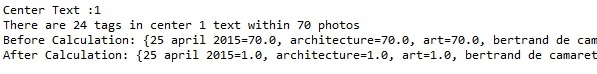
\includegraphics[width=50cm,bb=0 0 1820 73]{centroid.jpg}
	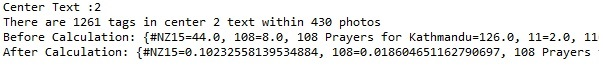
\includegraphics[width=50cm,bb=0 0 1820 73]{centroid2.jpg}
	\caption{Centroids Keywords from the appreciation}
	{\footnotesize Sample clusters tags data and weighted tags from application. Where the \textit{Center Text :1} is the first cluster and \textit{Center Text :2} is the second cluster. The line \textit{Before Calculation} and \textit{After Calculation} show the before and after the average calculation.}
\end{figure}

\pagebreak
}
\section{Experiment} \label{sec-evaluation}
In this section, we examine the performance of the proposed method, focusing on its effectiveness and efficiency. 
Specifically, we answer:
\begin{itemize}
\item How does the proposed Social Image Similarity function perform? 
We answer this by investigate the efficiency of the SIS-based clustering models,
the effect of cluster numbers with different types of clustering techniques,
and the effect of hash index. 
\item How effective and efficient of the proposed boundary-based change detection method (\emph{BBCD})?
We compare \emph{BBCD} with existing state-of-the-art algorithms, the shape base change detection(\textit{SBCD})~\cite{rs2051217}. 
\end{itemize}
\subsection{Experimental Setup}
The dataset we experimented with is collected from Flickr by focusing on images relevant to the \textit{Nepal earthquake}, which is also known as \textit{Gorkha earthquake}, in 2015.
Finally, 10,000 images are collected, which include images \emph{before} and \emph{after} the earthquake. 
The ground-truth is manually identified by the authors of this paper via careful comparison of all \emph{before} and \emph{after} images. 
Specifically, for a \emph{ground-truth}, both \emph{before} and \emph{after} image have to contain at least one same building, but the corresponding image contents, angles, resolutions, colours and light effects could be different. 
This would allow the proposed method to analyse whether the before and the after images are taken in the same location and building. 

We conduct the efficiency experiments on 10000 after and before the earthquake images and their features. 4000 after and before the earthquake images are collected for the effectiveness experiment. 
\yongli{this is confusing. How many images you collected? 10000 + 4000? or the 4000 is in the 10000 actually? why do effectiveness only on 4000? for time reason?}
\subsection{Measure metrics}
To evaluate the effectiveness of algorithms, 
we used two metrics in \cite{Zhou:2014:EDO:2628707.2628786}, 
the probability of miss detection and false alarm (\textit{Pmiss} and \textit{Pfa}). 
Specifically, the \emph{missed detection} mean that the algorithm fails to detect the ground-truth, and the \emph{false alarm} means the detection of non-target pairs. 
$Pmiss$ and $Pfa$ are defined as follows: 
\begin{equation}
Pmiss = \frac{number of missed detections}{number of ground truth}
\end{equation} 
\begin{equation}
Pfa = \frac{false alarms}{non targets }
\end{equation} 
a small value of \textit{Pmiss} and \textit{Pfa} means better effectiveness. 

The evaluation of efficiency includes two parts: 1) number of clusters, 
and 2) comparison with the existing damage detection algorithms.
Specifically, 
for number of clusters part test, 
it is expected to obtain the best cluster numbers to achieve the smallest \textit{Pmiss} and \textit{Pfa}.
We evaluate the efficiency of the proposed approach in terms of the overall time cost of clustering and hash index. 
We also evaluate the time cost of \textit{BBCD} and \textit{SBCD}, 
and to make the comparison more precise, we only compare the after the image matching time cost for change detection. 
Experiment are conducted on [machine information]...
\yongli{The above paragraph is very confusing, and please double check I rewrite what you want to present correctly. }
\subsection{Effectiveness}
We first examine the effect of number of cluster in \textit{SIS-based clustering} and \textit{OOS+LIP-IS}. 
After that, we compare the proposed approach with \textit{SBCD} by performing the change detection over the collected Flickr image datasets.

\subsubsection{Effect of clustering}

\subsubsection{Effectiveness comparasion}
Comparing with existing technique
We compare our \textit{DTW + change detection} with \textit{SBCD} used in \cite{rs2051217}. We assume 20\% of the building collapse are significant damage, we set the threshold of the unchanged building for the \textit{SBCD} as 80\%.
In \textit{SBCD} they did not perform the actual building matching. Therefore, in this test we selected 10 ground truth pairs(having similar angle) and 5 non ground truth pairs, which are paired by the \textit{OOS+LIP-IS}. 
comparing with shape-based approach. (in paper: \textbf{automatic detection of buildings and changes in buildings for updating of maps})

by varying the dataset size from small to big, test the probability of missed detection and probability of false alarm at each dataset size point


\subsection{Efficiency}

\subsubsection{Effect of different clustering techniques}
\subsubsection{Effect of hashing index}

\subsubsection{Efficiency comparison}

Detection efficiency by varying data size

this is only for comparing our boundary-based approach and existing shape-based approach.

\end{document}

